\documentclass{article}
%%%%%%%%%%%%%%%%%%%%%%%%%%%%%%%%%%%%%%%%%%%%%%%%%%%%%%%%%%%%%
% Lecture Specific Information to Fill Out
%%%%%%%%%%%%%%%%%%%%%%%%%%%%%%%%%%%%%%%%%%%%%%%%%%%%%%%%%%%%%
\newcommand{\LectureTitle}{L24: Image Capture}
%\newcommand{\LectureDate}{\today}
\newcommand{\LectureDate}{March 27, 2015}
\newcommand{\LectureClassName}{CS 557}
\newcommand{\LatexerName}{Peter Henderson}
%%%%%%%%%%%%%%%%%%%%%%%%%%%%%%%%%%%%%%%%%%%%%%%%%%%%%%%%%%%%%

% Change "article" to "report" to get rid of page number on title page
\usepackage{amsmath,amsfonts,amsthm,amssymb}
\usepackage{setspace}
\usepackage{Tabbing}
\usepackage{fancyhdr}
\usepackage{lastpage}
\usepackage{extramarks}
\usepackage{chngpage}
\usepackage{soul,color}
\usepackage{mathtools}
\usepackage{graphicx,float,wrapfig}
\usepackage{afterpage}
\usepackage{abstract}
\usepackage{pgfplots}
\usepackage{caption}
\usepackage{listings}
\usepackage{url}

% In case you need to adjust margins:
\topmargin=-0.45in
\evensidemargin=0in
\oddsidemargin=0in
\textwidth=6.5in
\textheight=9.0in
\headsep=0.25in
\tikzstyle{cnstyle}=[domain=0:1, samples=100, ultra thick]

% Setup the header and footer
\pagestyle{fancy}
\lhead{\LatexerName}
\chead{\LectureClassName: \LectureTitle}
\rhead{\LectureDate}
\lfoot{\lastxmark}
\cfoot{}
\rfoot{Page\ \thepage\ of\ \pageref{LastPage}}
\renewcommand\headrulewidth{0.4pt}
\renewcommand\footrulewidth{0.4pt}

%%%%%%%%%%%%%%%%%%%%%%%%%%%%%%%%%%%%%%%%%%%%%%%%%%%%%%%%%%%%%
% Some tools
\newcommand{\enterTopicHeader}[1]{\nobreak\extramarks{#1}{#1 continued on next page\ldots}\nobreak
                                    \nobreak\extramarks{#1 (continued)}{#1 continued on next page\ldots}\nobreak}
\newcommand{\exitTopicHeader}[1]{\nobreak\extramarks{#1 (continued)}{#1 continued on next page\ldots}\nobreak
                                   \nobreak\extramarks{#1}{}\nobreak}

\newlength{\labelLength}
\newcommand{\labelAnswer}[2]
  {\settowidth{\labelLength}{#1}
   \addtolength{\labelLength}{0.25in}
   \changetext{}{-\labelLength}{}{}{}
   \noindent\fbox{\begin{minipage}[c]{\columnwidth}#2\end{minipage}}
   \marginpar{\fbox{#1}}

   % We put the blank space above in order to make sure this
   % \marginpar gets correctly placed.
   \changetext{}{+\labelLength}{}{}{}}

\setcounter{secnumdepth}{0}
\newcommand{\TopicName}{}
\newcounter{TopicCounter}
\newenvironment{Topic}[1][Problem \arabic{TopicCounter}]
  {\stepcounter{TopicCounter}
   \renewcommand{\TopicName}{#1}
   \section{\TopicName}
   \enterTopicHeader{\TopicName}}
  {\exitTopicHeader{\TopicName}}

\setcounter{secnumdepth}{0}
\newcommand{\ExampleSectionName}{}
\newcounter{ExampleSectionCounter}[TopicCounter]
\newenvironment{ExampleSection}[1][Example \arabic{ExampleSectionCounter}]
  {\stepcounter{ExampleSectionCounter}
   \renewcommand{\ExampleSectionName}{#1}
   \section{\ExampleSectionName}
   \enterTopicHeader{\ExampleSectionName}}
  {\exitTopicHeader{\ExampleSectionName}}

\setcounter{secnumdepth}{0}
\newcounter{ExampleBoxCounter}[TopicCounter]
\newcommand{\examplebox}[1]
  {
  % We put this space here to make sure we're disconnected from the previous
   % passage
   \stepcounter{ExampleBoxCounter}
   \noindent\fbox{\begin{minipage}[c]{\columnwidth}#1\end{minipage}}\enterTopicHeader{\ExampleSectionName}\exitTopicHeader{\ExampleSectionName}\marginpar{\fbox{\#\arabic{ExampleBoxCounter}}}
   % We put the blank space above in order to make sure this
   % \marginpar gets correctly placed.
   \vskip10pt
   }

\renewcommand{\contentsname}{{\normalsize Topics Covered}}
\renewcommand{\abstractname}{\LectureTitle\ Summary}
\renewcommand{\absnamepos}{flushleft}

\pgfplotsset{vasymptote/.style={
    before end axis/.append code={
        \draw[densely dashed] ({rel axis cs:0,0} -| {axis cs:#1,0})
        -- ({rel axis cs:0,1} -| {axis cs:#1,0});
    }
}}

%%%%%%%%%%%%%%%%%%%%%%%%%%%%%%%%%%%%%%%%%%%%%%%%%%%%%%%%%%%%%

\begin{document}
\begin{spacing}{1.1}
\newpage

% When topics are long, it may be desirable to put a \newpage or a
% \clearpage before each Topic environment
%\newpage
\begin{Topic}[Image Capture \Roman{TopicCounter}]

As we have seen, in computer graphics, the projection surface is in front of the viewer. We were thinking of the viewer as looking through a window. In real cameras and eyes, images are formed behind the centre of projection (the light goes through a pinhole and is projected on a sensor plane, like your rods/cones or a camera's sensors behind the pinhole, not in front as is assumed in graphics).

\subsection{Aperture}
Real cameras (and eyes) have a finite aperture, not a pinhole. The diameter $A$ of the aperture can be varied to allow more or less light to reach the image plane. Similarly, the aperture in our eyes can vary (pupil dilation).

\subsection{Lens}
Cameras (and eyes) also have a lens (cornea) that focuses the light. A lens will bend the light such that if you have parallel rays, the lens will redirect those rays to some convergent point on the projection plane behind the lens.

For any point $(x_0, y_0, z_0)$, there is a corresponding point $(x_1, y_1, z_1)$, called the conjugate point. All the rays that leave $(x_0, y_0, z_0)$ and pass through the lens will converge on $(x_1, y_1, z_1)$ on the projection plane.

For any distance between the lens and sensor plane, some scene points will be in focus and some will be blurred. The amount of blur depends on the distance from the focal plane in the scene. So basically, rays that are bent by the lens and converge exactly on or near the projection plane are in focus. Rays that converge outside of the projection plane are blurred.

\subsection{Depth of Field}
\textit{Depth of field} is the range of depths that are pretty much in focus (their blur width is less than the distance between pixels).

\subsection{How to render image blur?}

To make images look realistic, you need to add some blur.\footnote{\url{http://http.developer.nvidia.com/GPUGems/gpugems_ch23.html}}

\subsubsection{Method I: Ray Tracing (Cook et al.) 1984}
For each point on the image plane, trace rays back through the lens into the scene. Compute the average of RGB values of all these rays. So you actually have a physics model for the lens which alters the ray paths, and you send a bunch of rays through the lens for each pixel and average them.

\subsubsection{Method 2: Accumulation buffer (Haeberli and Akeley 1990)}
Render the scene in the standard OpenGL way, from different camera positions within the aperture. Each of these images needs to be scaled and translated on the image plane. Then, sum up all the images.

\subsection{Camera Settings}

Define $f$ as your focal length (the distance from the lens to the projection plane). The total light reaching each point on the image plane depends on the intensity of the incoming light, and on the angle of the cone of rays which depends on the aperture. There is also a proportionality factor.

$$ E(x,y) = L(\vec{l})*\text{angleOfConeOfRays}(x)$$

$L(\vec{l})$ is the intensity of the light in direction l. There is a colour (wavelength) aspect also, but ignored for simplification.

``Solid Angle'' is a 2D angle (i.e. have a hemisphere of directions you can go in). It is defined to be the area of a unit hemisphere (radius 1) covered by the angle. Angle has units radians (or degrees). Solid angle has units ``steradians''. (e.g. You can talk about the solid angle of the sun or moon.)

Angular width of the lens as seen from the sensor is $\frac{A}{f}$. The units are radians.

(Solid) angleOfConeOfRays is proportional to: $(\frac{A}{F})^2$

The total light reaching each point on the image plane (per unit time) is thus as follows:

$$ E(x,y) = L(\vec{l})*(\frac{A}{f})^2$$

Here $t$ is the amount of time exposed to the light.

\subsubsection{F-number (definition)}

F-number (definition) $= \frac{f}{A}$ Since f / A (or its inverse) is fundamental to determining how much light reaches the image plane, this quantity is given a name. On typical cameras, the user can vary f-number: $\sqrt{2}, \sqrt{4}, \sqrt{8}, \sqrt{16}, \dots$. The mechanism for doing this is usually to vary the aperture. It is also possible to fix the aperture and vary the focal length.

\subsubsection{What happens when we vary the focal length?}
When you increase the distance (f) to the sensor plane, then you have a ``telephoto'' lens and your field of view is decreased. The image is also darker for the larger focal length. Why? Because the angle of the lens is smaller when viewed from a point on the sensor and thus less light gets in.

\subsubsection{Shutter speed 1/t (t = time of exposure)}
Image intensity also depends on this factor. Typical $t = \frac{1}{2}, \frac{1}{4}, \frac{1}{8}, \dots$, so shutter speeds $=2, 4, 8, \dots$. Shutter speed affects motion blur. There are some subtle features of motion blur however, demonstrated with billiards by Cook et al. (1984)\footnote{\url{http://graphics.pixar.com/library/DistributedRayTracing/paper.pdf}}.

\subsubsection{Exposure}
Exposure is a non-linear transformation $T(E(x,y)*t)=\{0, 1, \dots, 255\}$ and it saturates at 255. As we will see, it is useful to re-draw camera response curve as a function of log exposure.
\begin{center}
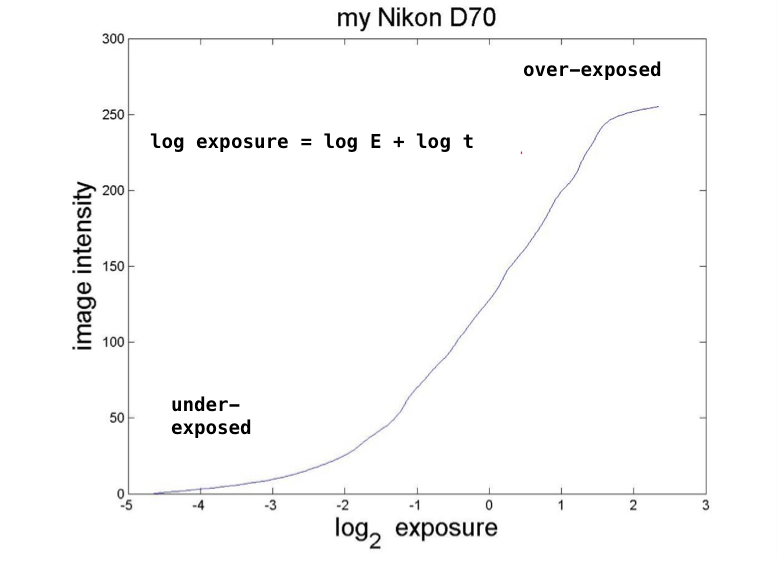
\includegraphics[scale=0.25]{images/exposure_graph}
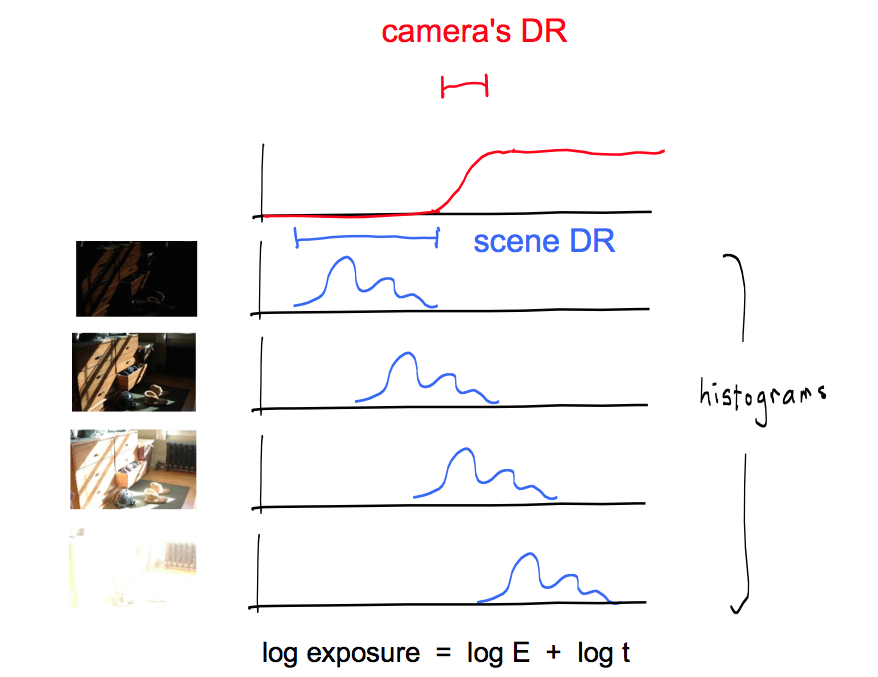
\includegraphics[scale=0.25]{images/dynamic_ranges}
\end{center}


\subsection{High Dynamic Range (HDR) Imaging}
Choosing the right exposure is hugely important and difficult. This problem is exacerbated by the fact that there's a huge range of lighting in natural scenes. To capture a high dynamic range with a low dynamic range camera, you take a bunch of pictures at different exposures and then combine them according to overall range of scene values.

\subsubsection{Dynamic Range}
\textit{Dynamic range} of a signal is the ratio of the maximum value to the minimum value. If we look at log(signal), then dynamic range is a difference, max - min. A typical scene has a dynamic range of luminances that is much greater than the dynamic range of exposures you can capture with a single image in your camera.

\subsubsection{How to compute camera response curve $T$?}
(Debevec and Malik 1997) \footnote{\url{http://www.pauldebevec.com/Research/HDR/debevec-siggraph97.pdf}}
\begin{itemize}
\item Take multiple exposures by varying shutter speed
\item Perform a ``least squares'' fit to a model of $T$. (This requires making a few reasonable assumptions about the model e.g. monotonically increasing, smooth, goes from 0 to 255.)
\item Option: compute separate models for RGB
\end{itemize}

\subsubsection{Computing a high dynamic range (HDR) image}
Given function $T$ for a camera, and given a set of new images $I_t(x,y)$ obtained for several shutter speeds, $1/t$,

$$E_t(x,y) = \frac{T^{-1}(I_t(x,y))}{t}$$

Use the estimate $E_t(x,y)$ for which $ 0 << I_t(x,y) << 255$ where the $T$ curve is most reliable.
\subsubsection{How to view a HDR image on a low dynamic range (LDR) display?}
This is the problem of ``tone mapping''. The simplest method is to compute $\log E(x,y)$ and scale values to [0, 255].

Tone mapping is a classical problem in painting/drawing. How to depict a HDR scene on a LDR display/canvas/print? Even painters in previous centuries have been trying to do this. (Typical dynamic range of paint/print is only about 30:1.) HDR has always been an issue in classical photography (e.g. Ansel Adams, techniques for ``burning and dodging'' prints).

\textit{Burning and dodging} means that in the light room you expose different parts of the image for various amounts of time.

HDR images can now be made with consumer level software.

\end{Topic}

\end{spacing}
\end{document}